\begin{figure}

  \setlength{\unitlength}{\textwidth}

  \begin{picture}(1,0.6)(0,0.8)
  
  
    % % %90
    \put(0.015,1.15){\includegraphics[width=0.5\unitlength]{./chapter-frequnecy-response/fnp/vel_time_history_1000.eps}}
    \put(0.495,1.15){\includegraphics[width=0.5\unitlength]{./chapter-frequnecy-response/fnp/vel_time_history_0001.eps}}
      \put(0.025,0.86){\includegraphics[width=0.496\unitlength]{./chapter-frequnecy-response/fnp/theta_time_history_1000.eps}}
      \put(0.495,0.86){\includegraphics[width=0.495\unitlength]{./chapter-frequnecy-response/fnp/theta_time_history_0001.eps}}
 	\put(0.01,0.98){ \large $\theta$} 
 	\put(0.01,1.28){ \large $\dot{y}$} 	
% 	\put(0.56,1.02){ $\theta$}
 	
 	
 	  \put(0.26,1.12){ $\displaystyle\frac{tU}{D}$} 	
 	  \put(0.75,1.12){ $\displaystyle\frac{tU}{D}$}
        \put(0.26,0.83){ $\displaystyle\frac{tU}{D}$} 	
        \put(0.75,0.83){ $\displaystyle\frac{tU}{D}$}
        
        
        \put(0.13,1.35){(a)}
        \put(0.61,1.35){(b)}
        \put(0.1,1.06){(c)}
        \put(0.5689,1.06){(d)}
         
      \end{picture}

  \caption{Time histories of $\dot{y}$ and $\theta$ at $\massdamp=0.2$ and $\ustar=40$  obtained from the QSS model . The time histories presented for : (a)  and (c) at $\massstiff=1000$; (b) and (d) at $\massstiff=0.001$ representing the two regions of frequency response. It is clearly evident that as \massstiff\ decreases the system becomes non-sinusoidal,}
    \label{fig:velocity-signal}
\end{figure}
